Harold R. Henry \cite{Henry60} \cite{Henry64} considered the problem of seawater intrusion into
coastal aquifers for the case of an isotropic homogeneous confined aquifer, in which there is a
steady seaward flow of freshwater. A constant flux of freshwater is applied to the inland boundary,
while a body of higher density seawater is on the seaward side. Seawater therefore, intrudes from
the seaward boundary towards the inland boundary until an equilibrium is reached between the heavier
seawater and the lighter freshwater recharge. The domain described above is depicted in
\autoref{fig:Domain}.

\begin{figure}[htp]
    \centering
    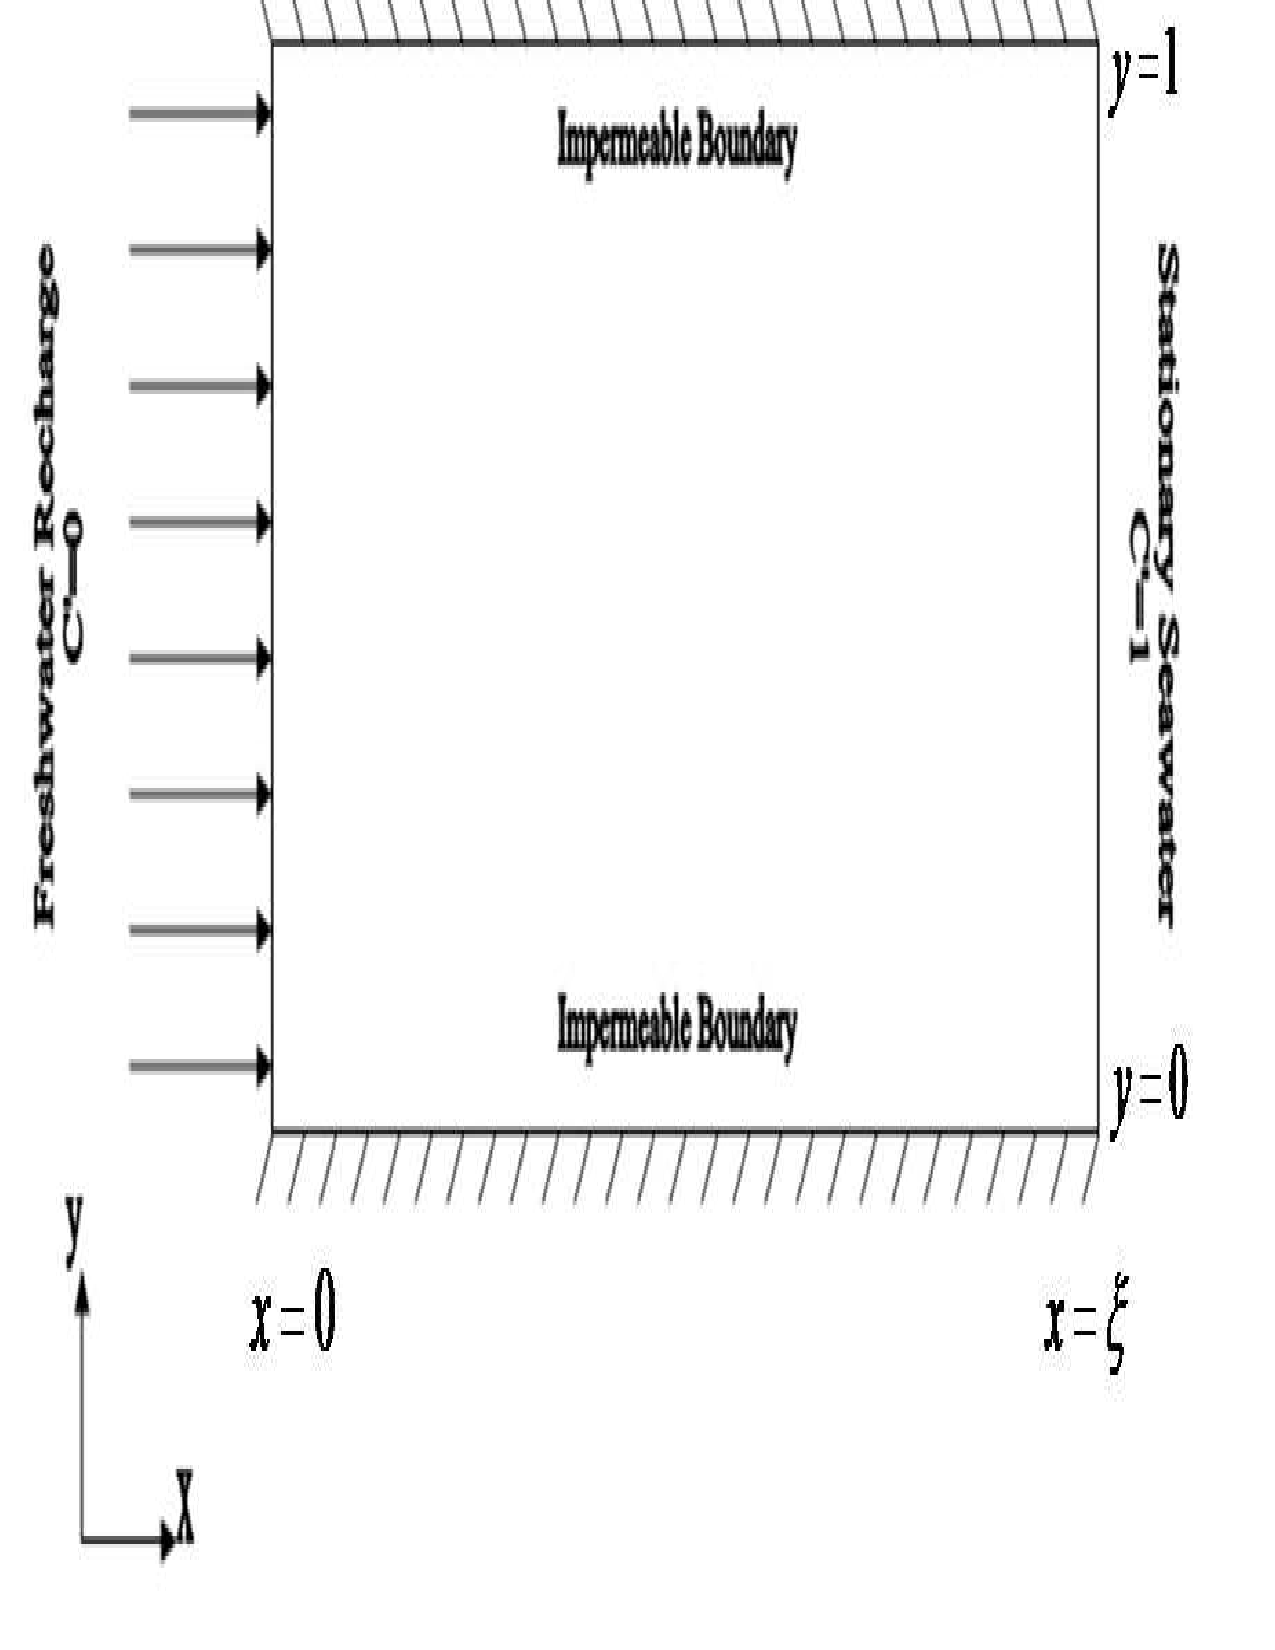
\includegraphics[scale=0.25]
    {image1}
    \caption{Depiction of 2D problem domain} \label{fig:Domain}
\end{figure}

Recently seawater intrusion has become a significant problem in coastal regions.  As populations
increase in these regions, natural recharge no longer counteracts the effects of withdrawals, and so
it is important to have a tool that can estimate the amount of seawater intrusion that may occur
with the continued withdrawal from coastal aquifers. Several numerical models have been developed to
address seawater intrusion in coastal aquifers, and so it is important to have an analytic solution
to use as a benchmark. The benchmarking of numerical code against analytic solutions is a necessary
step in verifying the correctness of the numerical approximations \cite{Simpson}.

Henry's Problem has been widely used as a benchmark case for numerical models of seawater intrusion.
Henry's Semi-Analytic Solution to Seawater Intrusion has been tempered by both the inability to use,
powerful computing technologies, which has become readily available to researchers, and a lack of a
sufficient number of Fourier coefficients, so as to ensure a smooth convergence. In fact, S\'egol
\cite{Segol} suggested that discrepancies between Henry and her own solutions may have been a result
of a lack of convergence in Henry's solution, due to a lack of powerful computing of the time, and
what S\'egol suggests was a poor initial guess. 

The method used by Henry to evaluate his Analytic solution has been plagued by the inability to use
a large number of Fourier coefficients, and therefore does not allow for realistic parameter values
Which have also prevented Henry's Solution from simulating narrow zones of dispersion. This is due
to Henry's method having a substantially low convergences rate with respect to the important
parameters $a$ and $b$.  Since Newton's method has a quadratic rate of convergence for well behaved
problems, one might expect greater ease in calculation for lower values of $a$ and $b$.  Therefore,
Newton's Method would address the convergence issues seen by Henry and others when trying to
simulate narrow zones of dispersion.

Newton's Method not only provides for a previously unused method for solving Henry's Problem, but
will also allow for more Fourier coefficients to be used in the solution, therefore allowing for a
more realistic solution sets. As more terms are used in a Fourier series the closer the numerical
solution comes to the true solution. Using Newton's method allows for the use of any number of
Fourier coefficients, and so it is now possible to evaluate Henry's Semi-Analytic Solution for
narrow zones of dispersion. The improved accuracy and the ability to simulate narrow zones of
dispersion will therefore improve Henry's Problem as a benchmark for comparison to numerical
solutions.

In this paper, we calculate the Fourier coefficients for the Henry problem by using Newton's method
to solve the nonlinear system of equations. Various truncations of the Fourier series are tested and
results are compared against the available result using Henry's method. Finally, $a$ and $b$ are
decreased to more realistic values and results are compared against numerical results from SUTRA
with similar parameter values.
